\subsection{Data Formats}

The data format is a part of the process of serialization, which enables data storage in a file, transmittal over the Internet, and reconstruction in a different environment. Serialization is the process of converting the state of an object into a stream of bytes, which later can be deserialized by rebuilding the stream of bytes to the original object. There are several data serialization formats; however, JavaScript Object Notation (JSON) and eXtensible Markup Language (XML) are the two most common data serialization formats. In this Section, we will discuss these formats. In the end, we will compare them and choose the format that meets the criteria of being compact, human-readable, and universal. 

\subsubsection{JSON}
JSON or JavaScript Object Notation is a light-weight and human-readable format that is commonly used for interchanging data on the web. The format is a text-based solution where the data structure is built on two structures: a collection of name-value pairs (known as objects) and ordered list of values (known as arrays). The JSON format is language-independent and the data structure universally recognized \cite{jsonorg, jsonvxml}. However, it is limited to a few predefined data types (i.e., string, number, boolean, object, array, and null), and extending the data type has to be done with the preliminary types. 

\begin{lstlisting}[language=json, caption={My Caption}, captionpos=b]
{
    "user": {
        "firstname": "Ola"
        "lastname": "Nordmann"
    }
}
\end{lstlisting}

\subsubsection{XML}
XML or eXtensible Markup Language is a simple and flexible format derived from Standard Generalized Markup Language (SGML), developed by the XML Working Group under the World Wide Web Consortium (W3C). An XML document consists of markups called tags, which are containers that describe and organize the enclosed data. The tag starts with \verb|<| and ends with \verb|>|; the content is placed between an opening tag and a closing tag (see listing). \cite{w3xml, jsonvxml} XML provides mechanisms to define custom data types, using existing data types as a starting point, making it extensible for future data. 

\begin{lstlisting}[language=json, caption={My Caption}, captionpos=b]
<user>
    <firstname>Ola</firstname>
    <lastname>Nordmann</lastname>
</user>
\end{lstlisting}

\subsubsection{Comparing}
We will compare JSON and XML features and performance with the study conducted by Saurabh and D’Souza \cite{jsonvxml}. There are apparent differences in the two data formats which affect the overall readability, extensibility, bandwidth performance, and ease of mapping. XML documents are easy to read, while JSON is obscure due to the parenthesis delimiters. XML allows for extended data types, while JSON is limited to a few data types. XML takes more bandwidth due to the metadata overhead, while JSON data is compact and use less amount of bandwidth.

Moreover, a few benchmarks were conducted to measure memory footprint and parsing runtime when serializing and deserializing JSON and XML data. From the conclusion,  in terms of memory footprint and parsing runtime, JSON performances better than XML but at the cost of readability and flexibility. While these format structures are applicable for transmitting data, choosing a format that is compact, human-readable, and a standard format that is extensible and scalable for future data is essential. In our design, we will be using the JSON format for transmission of the data.

\subsection{Data Entities}
Data entities are objects (e.g., things, persons, or places) that the system models and stores information about. Subsection about Storage introduces four data entities in our application (i.e., user, record, sample, and module). In Figure \ref{fig:dataentries}, the relation between the data entities are shown. Record and sample stores information about the recording, and are separated into two individual entities in order to reduce data redundancy and improve data integrity. Although, samples have a reference to its record so they can be associated with each other. A user stores biometrical information related to the user, the user in the application are patients. A record contains the state of the user's biometrical information at the time of the recording. In other words, the user's biometrical information can change over time (e.g.,  weight changes); therefore, capturing the exact biometrical information at the time of the recording is essential in the context of detecting sleeping illnesses with relation to the biometrical information.  A module is independent of the other data entities and stores information about the name and the package name of the module-application. The package name is used to locate and launch the module-application. 

In this Subsection, we will demonstrate the properties of each data entity in Nidra; storage structure of the entities, and illustration of the data structure for each entity.  

\begin{figure}
    \centering
    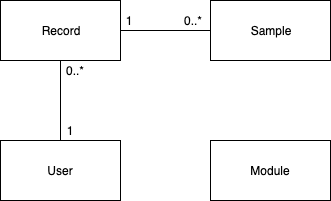
\includegraphics[scale=0.6]{images/DataEntries.png}
    \caption{Modules}
    \label{fig:dataentries}
\end{figure}

\subsubsection{Record}

A record is a table in the database that stores metadata related to the recording session. In Table 4.1, an illustration of the structure of a record is shown, with an entry of dummy data. In Nidra, the fields in the table for a record describe the data that is stored, which is separated into:
\begin{itemize}
	\item \verb|ID|: Unique identification of a record, also a primary key for the entry.
	\item \verb|Name|: A name of the record to easily recognize the recording.
	\item \verb|Description|: A summary over the recording session provided by the user It can be used to briefly describe how the recording session felt (e.g., any abnormalities during the sleep).
	\item \verb|MonitorTime|: The recording session duration in milliseconds.
	\item \verb|Rating|: Giving a rating on how the sleeping session felt, in a range between 0-5. 
	\item \verb|User|: User's biometriocal information encoded into a JSON string format, in order to capture the state of the user at recording. 
	\item \verb|CreatedAt|: Date of creation of the recording in milliseconds (since January 1, 1970, 00:00:00 GMT).
	\item \verb|UpdatedAt|: Date of update of the recording in milliseconds (since January 1, 1970, 00:00:00 GMT).
\end{itemize}


\begin{table}
\begin{center}
\scalebox{0.75}{
\begin{tabular}{ |c|c|c|c|c|c|c|c| } 
\hline
\textbf{id} & \textbf{name} & \textbf{description} & \textbf{monitorTime} & \textbf{rating} & \textbf{user} & \textbf{createdAt} & \textbf{updatedAt} \\
\hline
1 & Record \#1 & - & 5963088 & 2.5 & \{...\} & 1554406256000 & 1554406256000  \\ 
\hline
\end{tabular}}
\caption{Example entry in record table}
\end{center}
\end{table}


\subsubsection{Sample}
A sample is a single sensor reading containing data and metadata related to the recording session. Samples are stored separated from a record; however, they are linked with a field in the table.  In Table 4.1, an illustration of the structure of a sample is shown, with an entry of dummy data. In Nidra, the fields in the table for a sample describe the data that is stored accordingly to the data provided by Flow SweetZpot (ref), which are separated into:
\begin{itemize}
	\item \verb|ID|: Unique identification of a sample, also a primary key for the entry.
	\item \verb|RecordID|: An identification to its correlated record, also a foreign key. 
	\item \verb|ExplicitTS|: Timestamp of sample arrival based on the time in the sensor. 
	\item \verb|ImplicitTS|: Timestamp of sample arrival based on the time on the device. 
	\item \verb|Sample|: Sensor reading contains metadata and data according to Flow Sweetzpot. The sensor aggregates seven samples in a single sensor reading. 
\end{itemize}

\begin{table}
\begin{center}
\scalebox{0.60}{
\begin{tabular}{ |c|c|c|c|c| } 
\hline
\textbf{id} & \textbf{recordId} & \textbf{explicitTS} & \textbf{implicitTS} & \textbf{sample} \\
\hline
1 & 1 & 1554393086000 & 1554400286000 & Time=0ms, deltaT=100, data=1906,1891,1884,1881,1876,1718,1690 \\ 
\hline
\end{tabular}}
\caption{Example entry in sample table}
\end{center}
\end{table}


\subsubsection{Module}
A module is a table in the database that stores all modules installed by the user in the application. In Table 4.3, an illustration of the structure of a module is shown, with an entry of dummy data. In Nidra, the fields in the table contain the name of the module and the reference to the module and can be summarized as: 
\begin{itemize}
    \item \verb|ID|: Unique identification of a module, also a primary key for the entry.
    \item \verb|Name|: The name of the module-application.
    \item \verb|PackageName|: The package name of the module-application, such that it can be launched from Nidra. 
\end{itemize}

\begin{table}
\begin{center}
\scalebox{0.8}{
\begin{tabular}{ |c|c|c| } 
\hline
\textbf{id} & \textbf{name} & \textbf{packageName} \\
\hline
1 & OSA Predicter & com.package.osa\_predicter \\ 
\hline
\end{tabular}}
\caption{Example entry in module table}
\end{center}
\end{table}


\subsubsection{User}
The user of the application is the patient, which provides biometrical data (e.g., weight, height, and age). The biometrical data is part of the application to enrich the record. The record captures the biometrical state of the user at the time of the recording in the context of detecting sleeping illnesses with the relation to the biometrical data. In Nidra, the user entity is not a part of the database, but as an object stored in the device. The design decision of this choice is because the application is limited to one user at the time, and it makes it convenient to capture the state of the object of the given time of recording. It is possible to create a table in the database for the user entity, and for each time the user changes the biometrical data insert it is a separate entry in the database. The record could then have a reference to the latest user entry. However, that increases the complexity of the system, and as of now, the design of the application is to store the user's biometrical data into an object on the device. 

In Listing X, an illustration of the structure of a user is shown, with  dummy data. In Nidra, the user object is structured in a JSON format and contains biometrical data related to the user: 
\begin{itemize}
    \item \verb|Name|: Name of of the patient.
    \item \verb|Age|: Age of the patient.
    \item \verb|Gender|: Gender of the patient.
    \item \verb|Weight|: Weight of the patient in kilograms.
    \item \verb|Height|: Height of the patient in centimeters.
\end{itemize}

\begin{figure}
\begin{lstlisting}[language=json, caption={My Caption}, captionpos=b]
{
    "user": {
        "name": "Ola Nordmann",
        "age": 50,
        "gender": "Male",
        "height": 180,
        "weight: 60
    }
}
\end{lstlisting}
\end{figure}


\subsection{Data Packets}
Data packets are parcels of data that Nidra receives from external applications (e.g., sensor wrappers) or send to other application (e.g., sharing). From the design choice In the Section above, the format of all the desired data should be according to the JSON format.  In this Section.

\subsubsection{Sharing}

In Section (ref), a proposal to the structure of exporting and importing data is discussed. Two of the components (\verb|Parse Formatted Content| and \verb|Format File|) uses JSON to either encode or decode the data. Listing 4.3 illustrate the content of the encoded data from our application to gain a broader understanding of how the data exchange in sharing operates. The attractive attributes from the encoding are the record (ref) and the samples.  A record is an object that contains meta-data with name, number of samples, recording time, creation date, and user information. Samples are an array of objects that contains data, timestamp, and identification to correlated record. 

\begin{figure}
    
\begin{lstlisting}[language=json, caption={My Caption}, captionpos=b]
{
    "record":{  
        "id": 1,
        "name": "Record 1",
        "rating": 2.5,
        "description": "",
        "nrSamples": 6107,
        "monitorTime": 5963088,
        "createdAt": "Apr 4, 2019 9:30:56 PM",
        "updatedAt": "Apr 4, 2019 9:30:56 PM",
        "user": {  
            "age": 50,
            "createdAt": "---",
            "gender": "Male",
            "height": 180,
            "name": "Ola Nordmann",
            "weight": 60
        }
    },
    "samples": [  
        {  
            "explicitTS":"Apr 4, 2019 5:51:26 PM",
            "implicitTS":"Apr 4, 2019 7:51:26 PM",
            "recordId":1,
            "sample":"Time=0ms, deltaT=100, data=1906,1891,1884,1881,1876,1718,1690"
        },
        ...
    ]
}
\end{lstlisting}
\end{figure}

\subsubsection{Sensor Data}
Sensor data is data acquisition through the Data Dispatching (section background). The data format discussed in (section background). 